\documentclass[t]{beamer}

%% ----------------------------------------------------- PACKAGES ----------------------------------------------------- %%
\usepackage{coolPrez}
\bibliography{bibfile.bib}
%% ---------------------------------------------------- DOCUMENT ---------------------------------------------------- %%

\begin{document}

%% TITLE PAGE
\title[Learning from noisy demonstrations : a exploration/exploitation tradeoff]{Learning from noisy demonstrations : a exploration/exploitation tradeoff}
\author[]{Louis Faury\\ \vspace{5pt} \small{\textcolor{gray}{Advisors} : Mahdi Khoramshahi \& Andrew Sutcliffe}}
\institute[Semester Project at LASA]{Semester Project at LASA}
\titlegraphic{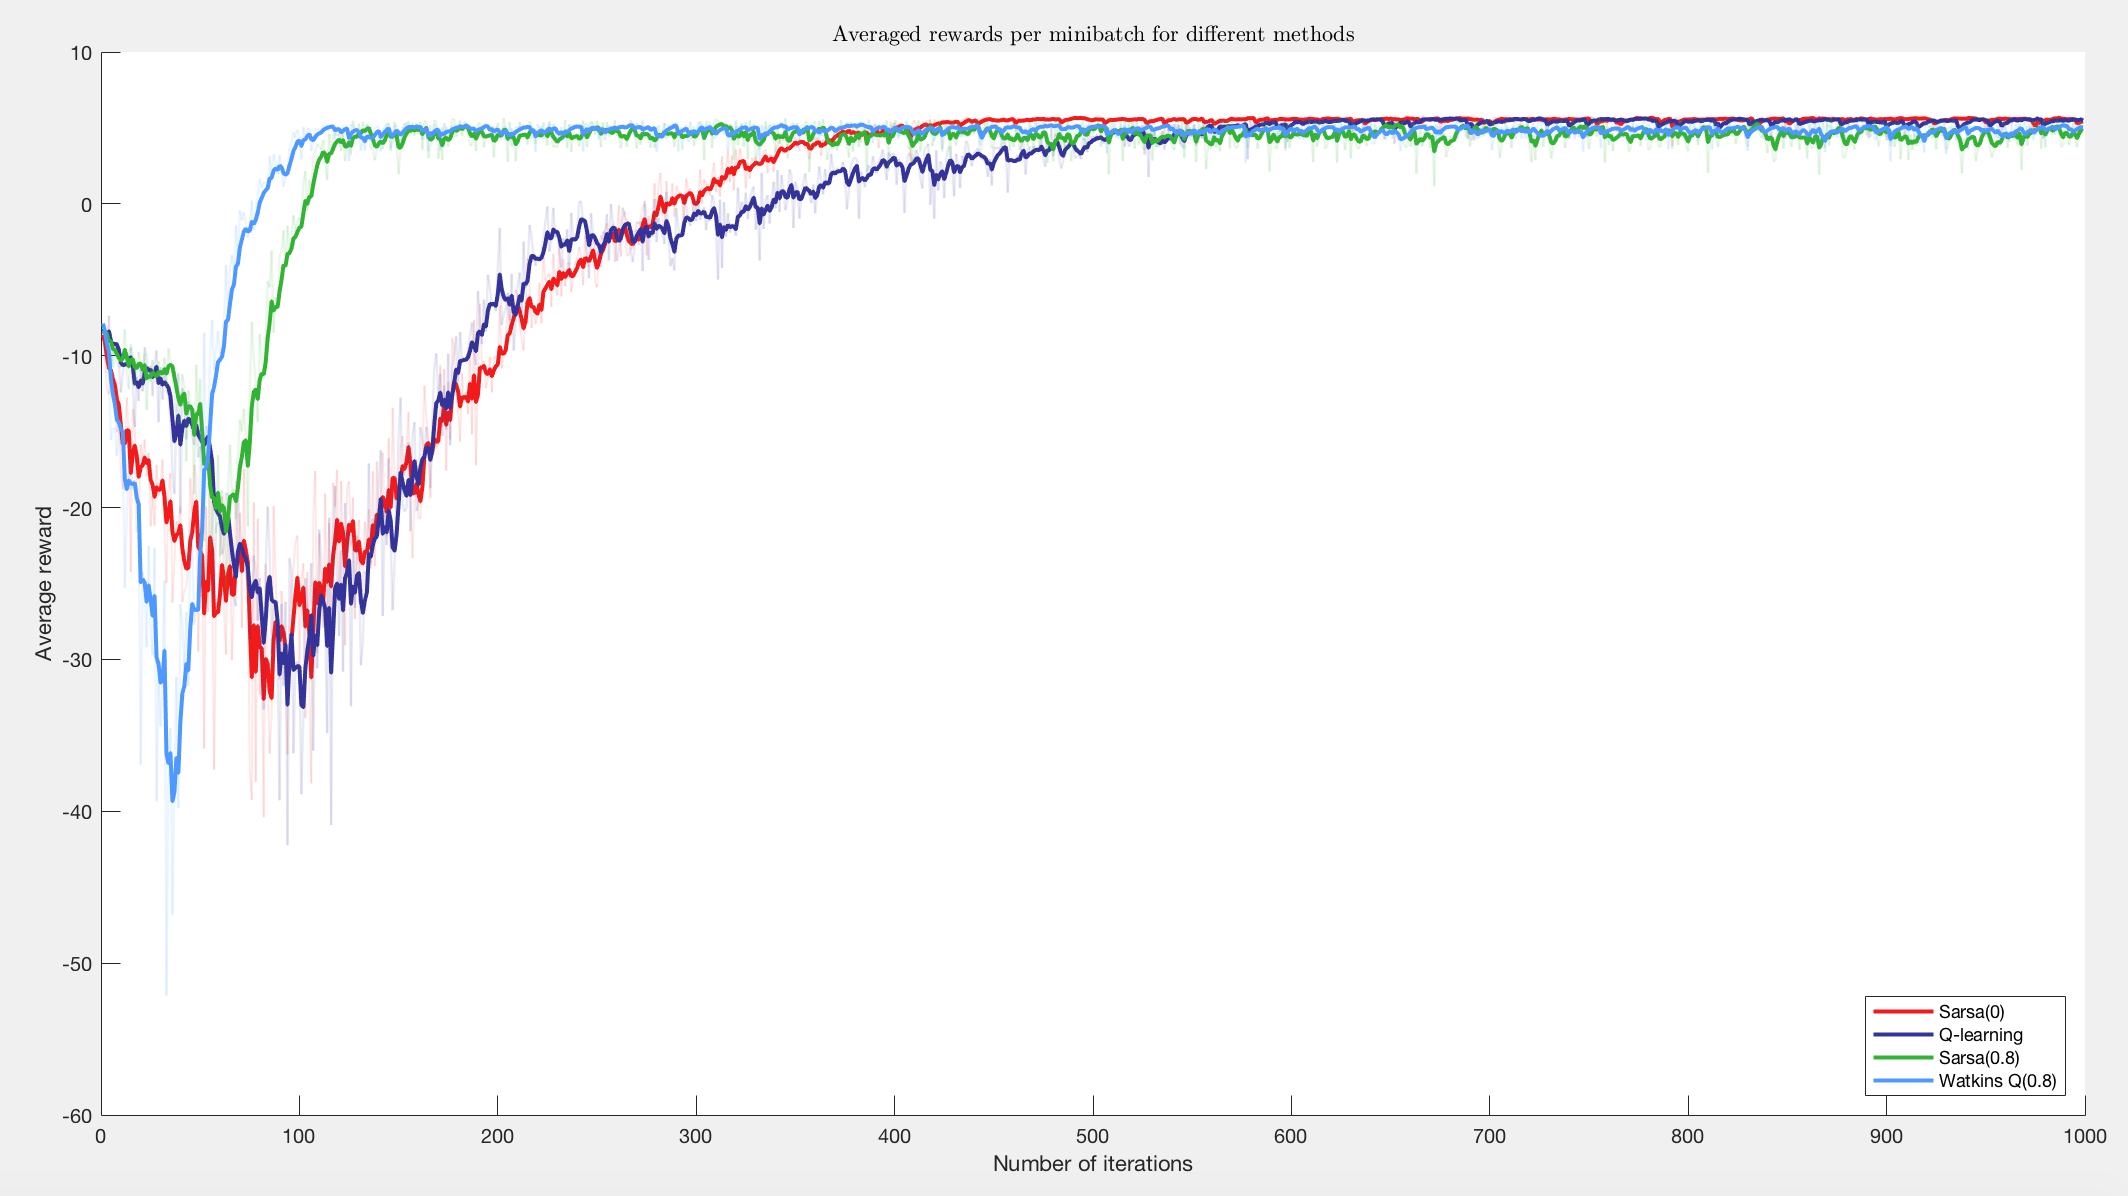
\includegraphics[width=0.7\linewidth]{titlepage_pic}}
\newenvironment{subenv}{\only{\setbeamercolor{local structure}{fg=red}}}{}

\titlepage

%1
\begin{frame}[t]
	\vspace{-3ex}
	\frametitle{Plan}
  	\tableofcontents
\end{frame}

\section{Motivations}
{
	\frame[t]
	{
		\vspace{20pt}
		\begin{itemize}
			\item For long and complex tasks : common machine learning algorithm are usually very slow to converge 
			\item Accelerate learning via prior knowledge of the environment or task : provide a \textcolor{red}{\textbf{demonstration}} of the task 
			\item Framework of \emph{learning from demonstration} (LfD) \footfullcite{Billard2016}
		\end{itemize}
		\vspace{25pt}
		\hspace{15pt} $\longrightarrow$ Ex. : robotic arm grabbing a cup \\
		\hspace{55pt} : maze solver 
	}
	\frame[t]
	{
		\vspace{10pt}
		\begin{itemize}
			\item How to take the teacher's demonstration into account?
				\begin{itemize}
					\item<sub@1> Exactly reproduce the teacher's actions 
					\item<sub@1> Use demonstration data to build a representation of the environment's dynamics
					\item<sub@1> \textbf{Use the teacher demonstration as an exploration baseline}
				\end{itemize}				
		\end{itemize}
		\vspace{15pt}
		\begin{itemize}
			\item Child learning to dance : first follow its dance teacher moves, before trying out new ones once he feels he has exploited the teacher's recommandation 
		\end{itemize}
		\hspace{50pt} $\color{red}\Rightarrow$ notion of \textcolor{red}{\textbf{compliance}} w.r.t the teacher. 
	}
	
		\frame[t]
	{
		\vspace{20pt}
		$\small\blacksquare$ \textbf{Goal} : 
			\begin{itemize}
				\item Introduce a theoretical framework for compliance-based learning 
				\item Grasp ideas and intuition about how such an approach can 
				\begin{itemize}
					\item<sub@1> Speed up the learning 
					\item<sub@1> Overcome some possible mentor's sub-optimality.  
					\item<sub@1> Generalize to \emph{transfer learning}
				\end{itemize}
			\end{itemize}
			in a \textbf{reinforcement learning framework}. 
			
		\vspace{20pt}
		$\small\blacksquare$ \textbf{Approach} :
			\begin{itemize}
				\item Create a simple but generic environment and task 
				\item Solve it using classical RL method 
				\item Implement compliant-based learning method 
				\item Compare them with classical methods, evaluate their pros and cons 
			\end{itemize}
	}
}

\section{Background}
{
	\subsection{Reinforcement learning}
	{
		\frame[t]
		{
			$\small\blacksquare$ \textbf{RL} :
			\begin{itemize}
				\item Framework in which an agent (or a learner) learns its actions from interaction with its environment
				\item The environment generates scalar values called rewards, that the agent is seeking to maximize over time.
			\end{itemize}
			\vspace{10pt}
			
			Under a Markovian asumption for the dynamics and reward system, the reinforcement learning problem can be formulated as a \emph{Markov Decision Process} : 
			\begin{equation}
				(\mathcal{S}, \mathcal{A}(\mathcal{S}), \mathcal{P}_{ss'}^a , \mathcal{R}_{ss'}^a)
			\end{equation}
			where : 
			\begin{equation}
				\begin{aligned}
					&\mathcal{P}_{ss'}^a = \underbrace{\mathbb{P}(s_{t+1}=s' \, \vert \, s_t=s,\, a_t =a )}_{dynamics}
\quad  & \mathcal{S} \text{ : state space}\\
					&\mathcal{R}_{ss'}^a = \underbrace{\E{r_t \, \vert \, s_{t+1}=s', \,s_t=s,\, a_t =a )}}_{immediate reward} \quad & \mathcal{A(\mathcal{S})} \text{ : action space}
				\end{aligned}
			\end{equation}
		}
		\frame[t]
		{
			$\small\blacksquare$ \textbf{RL} :
			\begin{itemize}
				\item Define state value and action value function under a policy (probabilistic decision rule) $\pi \, : \, \mathcal{S} \to \mathcal{A}$ : 
				\begin{equation}
					\begin{aligned}
						V^\pi(s) &= \E[\pi]{\sum_i \gamma^i r_{t+i+1}\, \vert s_t = s }\\
						Q^\pi(s,a) &= \E[\pi]{\sum_i \gamma^i r_{t+i+1}\, \vert s_t = s , a_t =a }\\
					\end{aligned}
				\end{equation}
			\item All algorithm computing optimal policies rely on various mix of a \textcolor{red}{\emph{Generalized Policy Iteration}} : 
				\begin{enumerate}
					\item[1.] Evaluate the current policy (DP,..)
					\item[2.] Improve the current policy (greedization) 
					\item[3.] Repeat
				\end{enumerate}
			\end{itemize}
		
		}
	}
		\subsection{Transfer learning}
	{
		\frame[t]
		{
			
		}
	}
}

\section{Approach}
{
	\subsection{A sandbox state space}
	{
		\frame[t]
		{
	
		}
	}
	\subsection{RL results}
	{
		\frame[t]
		{
	
		}
	}
	\subsection{Compliance based update rule}
	{
		\frame[t]
		{
	
		}
	}
	\subsection{Results}
	{
		\frame[t]
		{
	
		}
	}
}


%Bibliography
%\bibliography{bib.bib}

\end{document}